\documentclass[a4paper, 10pt]{article}
\usepackage[margin=1.5cm]{geometry} % 稍微缩小页边距以容纳更多图
\usepackage{tikz}
\usepackage{caption}
\usepackage{subcaption}
\usepackage{float}
\usetikzlibrary{arrows, decorations.pathmorphing, decorations.markings, shapes.geometric, calc, positioning}

\tikzset{
    node0/.style={circle, draw, fill=white, inner sep=0pt, minimum size=1.5mm},
    node1/.style={circle, draw, fill=black, inner sep=0pt, minimum size=1.5mm},
    reoEdge/.style={->, >=latex, thin},
    reoSpout/.style={<->, >=latex, thin},
    reoLossy/.style={->, >=latex, thin, dashed},
    reoWavy/.style={->, >=latex, thin, decorate, decoration={zigzag, amplitude=1mm, segment length=1.5mm, post length=1.5mm, pre length=1.5mm}},
}

% A. 基础连线类 (Sync, Lossy, Filter)  参数: #1=样式(可选), #2=起点, #3=终点, #4=标签文字(可选)
\newcommand{\drawLink}[4][reoEdge]{
    \draw[#1] (#2) -- node[above, font=\scriptsize] {#4} (#3);
}

% B. FIFO 类 (中间带方框)  参数: #1=起点, #2=终点, #3=方框内文字, #4=额外样式(可选,如 dashed)
\newcommand{\drawFIFO}[4][]{
    \draw[reoEdge, #1] (#2) -- node[midway, sloped, allow upside down, draw, fill=white, rectangle, minimum width = 6mm, minimum height = 2mm, inner sep=1pt, font=\tiny] {#4} (#3);
}

% C. Drain 类 (两头向中间汇聚)  参数: #1=起点1, #2=起点2, #3=汇聚点/符号位置(通常是这两个点的中点), #4=中心符号(如 ||)
\newcommand{\drawDrain}[5]{
    % 计算中点
    \coordinate (mid1) at ($(#1)!0.4!(#2)$);
    \coordinate (mid) at ($(#1)!0.5!(#2)$);
    \coordinate (mid2) at ($(#1)!0.6!(#2)$);
    % 画两段箭头指向中点
    \draw[->, >=latex, thin] (#1) -- (mid1);
    \draw[thin] (mid1) -- (mid);
    \draw[thin] (mid) -- (mid2);
    \draw[->, >=latex, thin] (#2) -- (mid2);
    % 画中心符号
    \node at (mid) [font=\tiny, inner sep=1pt] {#3};
    \node at (mid1) [font=\tiny, inner sep=1pt] {#4};
    \node at (mid2) [font=\tiny, inner sep=1pt] {#5};
    % 实际上 Drain 并没有显式的 Sink 节点,这里 #3 只是为了兼容位置逻辑,或者如果不画节点只画线
}

% D. Spout 类 (一点分发给两点)  参数: #1=源点, #2=终点1, #3=终点2, #4=线样式
\newcommand{\drawSpout}[5]{
    % 计算中点
    \coordinate (mid1) at ($(#1)!0.4!(#2)$);
    \coordinate (mid) at ($(#1)!0.5!(#2)$);
    \coordinate (mid2) at ($(#1)!0.6!(#2)$);
    % 画两段箭头指向中点
    \draw[->, >=latex, thin] (mid1) -- (#1);
    \draw[thin] (mid1) -- (mid);
    \draw[thin] (mid) -- (mid2);
    \draw[->, >=latex, thin] (mid2) -- (#2);
    % 画中心符号
    \node at (mid) [font=\tiny, inner sep=1pt] {#3};
    \node at (mid1) [font=\tiny, inner sep=1pt] {#4};
    \node at (mid2) [font=\tiny, inner sep=1pt] {#5};
    % 实际上 Drain 并没有显式的 Sink 节点,这里 #3 只是为了兼容位置逻辑,或者如果不画节点只画线
}

% E. Timer 类 (中间带圆角框)  参数: #1=起点, #2=终点, #3=延迟时间 t
\newcommand{\drawTimer}[3]{
    \draw[reoEdge] (#1) -- node[draw, fill=white, rectangle, rounded corners=2pt, minimum size=3.5mm, inner sep=1pt, font=\tiny] (timerbox) {#3} (#2);
}

% F. 复杂 Timer 类 (带控制端口 OFF/RESET/EXPIRE)  参数: #1=起点, #2=终点, #3=延迟时间 t, #4=控制类型(OFF/RST/EXP), #5=控制节点位置(above/below)
\newcommand{\drawComplexTimer}[5]{
    % 先画基础 Timer
    \draw[reoEdge] (#1) -- node[draw, fill=white, rectangle, rounded corners=2pt, minimum size=3.5mm, inner sep=1pt, font=\tiny] (timerbox) {#3} (#2);
    % 画控制端口
    \node (ctrl) [#5=0.5cm of timerbox, font=\tiny] {#4};
    \draw[->, >=latex, dashed] (ctrl) -- (timerbox);
}


% --- 1. Basic Channels ---
\newcommand{\chanSync}[2]{\drawLink{#1}{#2}{}}
\newcommand{\chanLossySync}[2]{\drawLink[reoLossy]{#1}{#2}{}}
\newcommand{\chanSyncDrain}[2]{\drawDrain{#1}{#2}{}{}{}} % 空心汇聚
\newcommand{\chanAsynDrain}[2]{\drawDrain{#1}{#2}{$||$}{}{}} % 带竖线汇聚
% --- 2. FIFO Variants ---
\newcommand{\chanFifoOne}[2]{\drawFIFO{#1}{#2}{}}          % Buffer size 1
\newcommand{\chanFifoN}[3]{\drawFIFO{#1}{#2}{$N=#3$}}      % Buffer size n
\newcommand{\chanFifoOneE}[3]{\drawFIFO{#1}{#2}{$#3$}}     % Initialized with e
\newcommand{\chanFifoNE}[4]{\drawFIFO{#1}{#2}{$#3$}}    % Initialized e with size n
% --- 3. Filter & Producer ---
\newcommand{\chanFilterP}[3]{\drawLink[reoWavy]{#1}{#2}{$P(#3)$}} 
\newcommand{\chanProducerP}[3]{\drawLink{#1}{#2}{Prod: $#3$}} 
% --- 4. Spouts ---
\newcommand{\chanSyncSpout}[2]{\drawSpout{#1}{#2}{}{}{}}
\newcommand{\chanAsynSpout}[2]{\drawSpout{#1}{#2}{$||$}{}{}}
% --- 5. Probabilistic/Faulty ---
\newcommand{\chanCptSync}[3]{\drawLink{#1}{#2}{$p=#3$}}       % Corrupting Sync
\newcommand{\chanRdmSync}[3]{\drawLink{#1}{#2}{#3}}         % Random Sync
\newcommand{\chanProbLossy}[3]{\drawLink[reoLossy]{#1}{#2}{$p=#3$}} % Probabilistic Lossy
\newcommand{\chanFtyFifoOne}[3]{\drawFIFO{#1}{#2}{Fty:$#3$}} % Faulty FIFO
\newcommand{\chanLossyFifoOne}[3]{\drawFIFO[dashed]{#1}{#2}{Lossy:$#3$}} % Lossy FIFO
% --- 6. Timers ---
\newcommand{\chanTimert}[3]{\drawTimer{#1}{#2}{#3}}
\newcommand{\chanOFFTimert}[3]{\drawComplexTimer{#1}{#2}{#3}{OFF}{above}}
\newcommand{\chanRSTTimert}[3]{\drawComplexTimer{#1}{#2}{#3}{RST}{above}}
\newcommand{\chanEXPTimert}[3]{\drawComplexTimer{#1}{#2}{#3}{EXP}{above}}

\title{Visualized Test Cases}
\date{}

\begin{document}

\maketitle

\section{Basic test cases}

\vspace{0.5cm}
\hrule
\vspace{0.5cm}

% ============================================================
% test_basic_01
% ============================================================
\subsection*{test basic 01}
\vspace{0.2cm}

\begin{minipage}{0.48\textwidth}
    \centering
    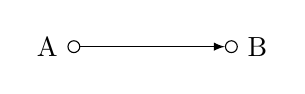
\begin{tikzpicture}[node distance=2cm]

        \node[node0, label=left:A] (A) at (0,0) {};
        \node[node0, label=right:B] (B) at (2,0) {};

        \chanSync{A}{B}

    \end{tikzpicture}
\end{minipage}
\hfill
\begin{minipage}{0.48\textwidth}
    \centering
    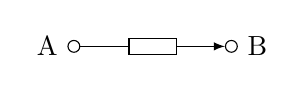
\begin{tikzpicture}[node distance=2cm]

        \node[node0, label=left:A] (A) at (0,0) {};
        \node[node0, label=right:B] (B) at (2,0) {};

        \chanFifoOne{A}{B}

    \end{tikzpicture}
    
\end{minipage}

\vspace{0.5cm}
\hrule
\vspace{0.5cm}

% ============================================================
% test_basic_02
% ============================================================
\subsection*{test basic 02}
\vspace{0.2cm}

\begin{minipage}{0.48\textwidth}
    \centering
    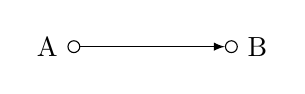
\begin{tikzpicture}[node distance=2cm]

        \node[node0, label=left:A] (A) at (0,0) {};
        \node[node0, label=right:B] (B) at (2,0) {};

        \chanSync{A}{B}

    \end{tikzpicture}
\end{minipage}
\hfill
\begin{minipage}{0.48\textwidth}
    \centering
    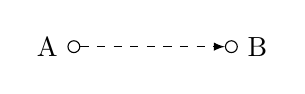
\begin{tikzpicture}[node distance=2cm]

        \node[node0, label=left:A] (A) at (0,0) {};
        \node[node0, label=right:B] (B) at (2,0) {};

        \chanLossySync{A}{B}

    \end{tikzpicture}
\end{minipage}

\vspace{0.5cm}
\hrule
\vspace{0.5cm}

% ============================================================
% test_basic_03
% ============================================================
\subsection*{test basic 03}
\vspace{0.2cm}

\begin{minipage}{0.48\textwidth}
    \centering
    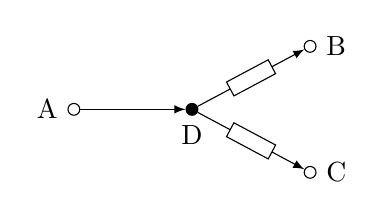
\begin{tikzpicture}[x=1.5cm, y=1cm]

        \node[node0, label=left:A] (A) at (0,0) {};
        \node[node1, label=below:D] (D) at (1,0) {};
        \node[node0, label=right:B] (B) at (2,0.8) {};
        \node[node0, label=right:C] (C) at (2,-0.8) {};
        
        \chanSync{A}{D}
        \chanFifoOne{D}{B}
        \chanFifoOne{D}{C}

    \end{tikzpicture}
\end{minipage}
\hfill
\begin{minipage}{0.48\textwidth}
    \centering
    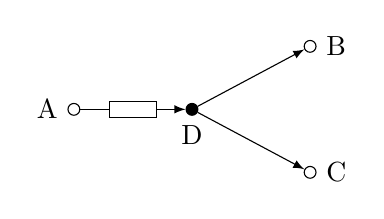
\begin{tikzpicture}[x=1.5cm, y=1cm]

        \node[node0, label=left:A] (A) at (0,0) {};
        \node[node1, label=below:D] (D) at (1,0) {};
        \node[node0, label=right:B] (B) at (2,0.8) {};
        \node[node0, label=right:C] (C) at (2,-0.8) {};
        
        \chanFifoOne{A}{D}
        \chanSync{D}{B}
        \chanSync{D}{C}

    \end{tikzpicture}
\end{minipage}

\vspace{0.5cm}
\hrule
\vspace{0.5cm}

% ============================================================
% test_basic_04
% ============================================================
\subsection*{test basic 04}
\vspace{0.2cm}

\begin{minipage}{0.48\textwidth}
    \centering
    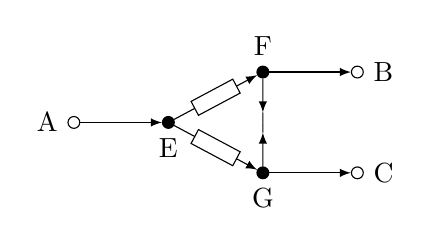
\begin{tikzpicture}[x=1.2cm, y=0.8cm]

        \node[node0, label=left:A] (A) at (0,0) {};
        \node[node1, label=below:E] (E) at (1,0) {};
        \node[node1, label=above:F] (F) at (2,0.8) {};
        \node[node1, label=below:G] (G) at (2,-0.8) {};
        \node[node0, label=right:B] (B) at (3,0.8) {};
        \node[node0, label=right:C] (C) at (3,-0.8) {};
        
        \chanSync{A}{E}
        \chanFifoOne{E}{F}
        \chanFifoOne{E}{G}
        \chanSyncDrain{F}{G}
        \chanSync{F}{B}
        \chanSync{G}{C}

    \end{tikzpicture}
\end{minipage}
\hfill
\begin{minipage}{0.48\textwidth}
    \centering
    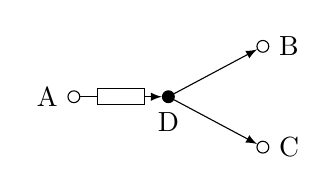
\begin{tikzpicture}[x=1.2cm, y=0.8cm]

        \node[node0, label=left:A] (A) at (0,0) {};
        \node[node1, label=below:D] (D) at (1,0) {};
        \node[node0, label=right:B] (B) at (2,0.8) {};
        \node[node0, label=right:C] (C) at (2,-0.8) {};
        
        \chanFifoOne{A}{D}
        \chanSync{D}{B}
        \chanSync{D}{C}

    \end{tikzpicture}
\end{minipage}

\vspace{0.5cm}
\hrule
\vspace{0.5cm}

% ============================================================
% test_basic_05
% ============================================================
\subsection*{test basic 05}
\vspace{0.2cm}

\begin{minipage}{0.48\textwidth}
    \centering
    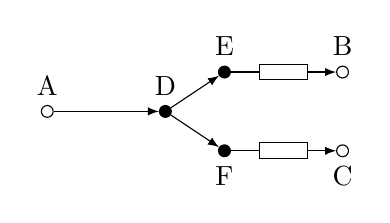
\begin{tikzpicture}[x=1.5cm, y=1cm]
        
        \node[node0, label=above:A] (A) at (0, -0.5) {};
        \node[node0, label=above:B] (B) at (2.5, 0) {};
        \node[node0, label=below:C] (C) at (2.5, -1) {};
        \node[node1, label=above:D] (D) at (1, -0.5) {};
        \node[node1, label=above:E] (E) at (1.5, 0) {};
        \node[node1, label=below:F] (F) at (1.5, -1) {};

        \chanSync{A}{D}
        \chanSync{D}{E}
        \chanSync{D}{F}
        \chanFifoOne{E}{B}
        \chanFifoOne{F}{C}

    \end{tikzpicture}
\end{minipage}
\hfill
\begin{minipage}{0.48\textwidth}
    \centering
    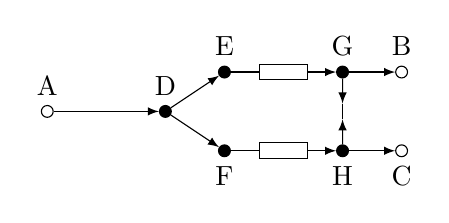
\begin{tikzpicture}[x=1.5cm, y=1cm]

        \node[node0, label=above:A] (A) at (0, -0.5) {};
        \node[node0, label=above:B] (B) at (3, 0) {};
        \node[node0, label=below:C] (C) at (3, -1) {};
        \node[node1, label=above:D] (D) at (1, -0.5) {};
        \node[node1, label=above:E] (E) at (1.5, 0) {};
        \node[node1, label=below:F] (F) at (1.5, -1) {};
        \node[node1, label=above:G] (G) at (2.5, 0) {};
        \node[node1, label=below:H] (H) at (2.5, -1) {};

        \chanSync{A}{D}
        \chanSync{D}{E}
        \chanSync{D}{F}
        \chanFifoOne{E}{G}
        \chanFifoOne{F}{H}
        \chanSyncDrain{G}{H}
        \chanSync{G}{B}
        \chanSync{H}{C}

    \end{tikzpicture}
\end{minipage}

\vspace{0.5cm}
\hrule
\vspace{0.5cm}

% ============================================================
% test_basic_06
% ============================================================
\subsection*{test basic 06}
\vspace{0.2cm}

\begin{minipage}{0.48\textwidth}
    \centering
    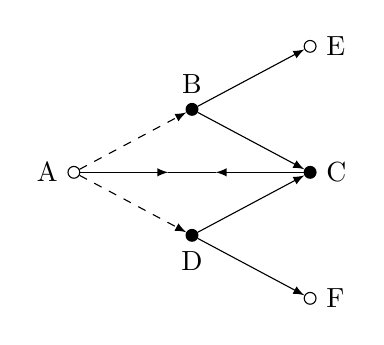
\begin{tikzpicture}[x=1.5cm, y=1cm]

        \node[node0, label=left:A] (A) at (0,0) {};
        \node[node1, label=above:B] (B) at (1,0.8) {};
        \node[node1, label=below:D] (D) at (1,-0.8) {};
        \node[node1, label=right:C] (C) at (2,0) {};
        \node[node0, label=right:E] (E) at (2,1.6) {};
        \node[node0, label=right:F] (F) at (2,-1.6) {};
        
        \chanLossySync{A}{B}
        \chanLossySync{A}{D}
        \chanSyncDrain{A}{C}
        \chanSync{B}{C}
        \chanSync{D}{C}
        \chanSync{B}{E}
        \chanSync{D}{F}

    \end{tikzpicture}
\end{minipage}
\hfill
\begin{minipage}{0.48\textwidth}
    \centering
    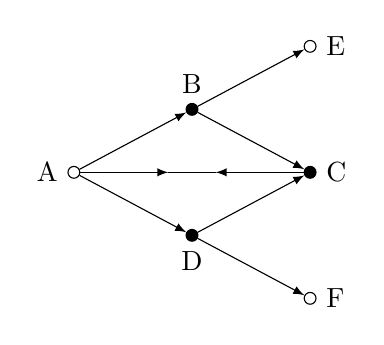
\begin{tikzpicture}[x=1.5cm, y=1cm]

        \node[node0, label=left:A] (A) at (0,0) {};
        \node[node1, label=above:B] (B) at (1,0.8) {};
        \node[node1, label=below:D] (D) at (1,-0.8) {};
        \node[node1, label=right:C] (C) at (2,0) {};
        \node[node0, label=right:E] (E) at (2,1.6) {};
        \node[node0, label=right:F] (F) at (2,-1.6) {};
        
        \chanSync{A}{B}
        \chanSync{A}{D}
        \chanSyncDrain{A}{C}
        \chanSync{B}{C}
        \chanSync{D}{C}
        \chanSync{B}{E}
        \chanSync{D}{F}

    \end{tikzpicture}
\end{minipage}

\vspace{0.5cm}
\hrule
\vspace{0.5cm}

% ============================================================
% test_basic_07
% ============================================================
\subsection*{test basic 07}
\vspace{0.2cm}

\begin{minipage}{0.48\textwidth}
    \centering
    \scalebox{0.85}{
    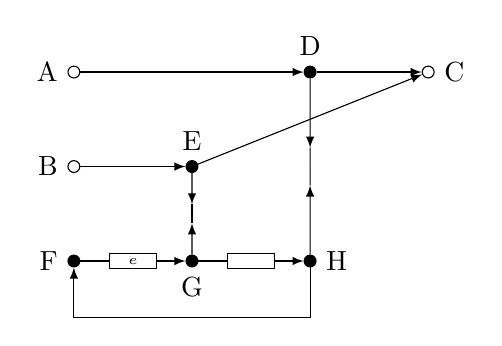
\begin{tikzpicture}[x=1.5cm, y=1.2cm]
        
        \node[node0, label=left:A] (A) at (0, 2) {};
        \node[node0, label=left:B] (B) at (0, 1) {};
        \node[node0, label=right:C] (C) at (3, 2) {};
        \node[node1, label=above:D] (D) at (2, 2) {};
        \node[node1, label=above:E] (E) at (1, 1) {};
        \node[node1, label=left:F] (F) at (0, 0) {};
        \node[node1, label=below:G] (G) at (1, 0) {};
        \node[node1, label=right:H] (H) at (2, 0) {};
        
        \chanSync{A}{D}
        \chanSync{B}{E}
        \chanSync{D}{C}
        \chanSync{E}{C}
        \chanFifoOneE{F}{G}{e}
        \chanFifoOne{G}{H}
        \draw[reoEdge] (H) -- ++(0, -0.6) -| (F);
        \chanSyncDrain{E}{G}
        \chanSyncDrain{D}{H}

    \end{tikzpicture}
    }
\end{minipage}
\hfill
\begin{minipage}{0.48\textwidth}
    \centering
    \scalebox{0.85}{
    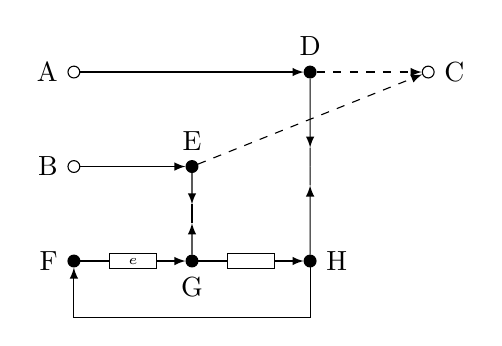
\begin{tikzpicture}[x=1.5cm, y=1.2cm]
        
        \node[node0, label=left:A] (A) at (0, 2) {};
        \node[node0, label=left:B] (B) at (0, 1) {};
        \node[node0, label=right:C] (C) at (3, 2) {};
        \node[node1, label=above:D] (D) at (2, 2) {};
        \node[node1, label=above:E] (E) at (1, 1) {};
        \node[node1, label=left:F] (F) at (0, 0) {};
        \node[node1, label=below:G] (G) at (1, 0) {};
        \node[node1, label=right:H] (H) at (2, 0) {};
        
        \chanSync{A}{D}
        \chanSync{B}{E}
        \chanLossySync{D}{C}
        \chanLossySync{E}{C}
        \chanFifoOneE{F}{G}{e}
        \chanFifoOne{G}{H}
        \draw[reoEdge] (H) -- ++(0, -0.6) -| (F);
        \chanSyncDrain{E}{G}
        \chanSyncDrain{D}{H}

    \end{tikzpicture}
    }
\end{minipage}

\vspace{0.5cm}
\hrule
\vspace{0.5cm}

% ============================================================
% test_basic_08
% ============================================================
\subsection*{test basic 08}
\vspace{0.2cm}

\begin{minipage}{0.48\textwidth}
    \centering
    \scalebox{0.85}{
    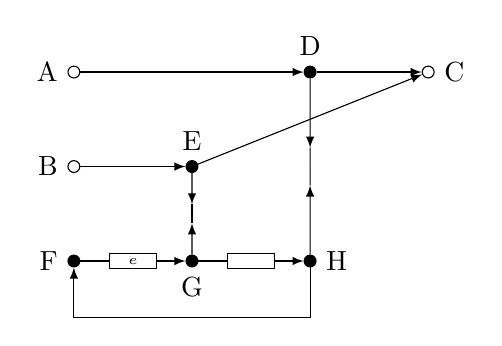
\begin{tikzpicture}[x=1.5cm, y=1.2cm]
        
        \node[node0, label=left:A] (A) at (0, 2) {};
        \node[node0, label=left:B] (B) at (0, 1) {};
        \node[node0, label=right:C] (C) at (3, 2) {};
        \node[node1, label=above:D] (D) at (2, 2) {};
        \node[node1, label=above:E] (E) at (1, 1) {};
        \node[node1, label=left:F] (F) at (0, 0) {};
        \node[node1, label=below:G] (G) at (1, 0) {};
        \node[node1, label=right:H] (H) at (2, 0) {};
        
        \chanSync{A}{D} \chanSync{B}{E}
        \chanSync{D}{C} \chanSync{E}{C}
        \chanFifoOneE{F}{G}{e} \chanFifoOne{G}{H}
        \draw[reoEdge] (H) -- ++(0, -0.6) -| (F);
        \chanSyncDrain{E}{G} \chanSyncDrain{D}{H}

    \end{tikzpicture}
    }
\end{minipage}
\hfill
\begin{minipage}{0.48\textwidth}
    \centering
    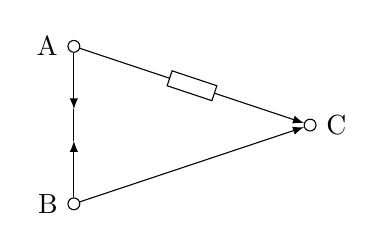
\begin{tikzpicture}[node distance=2cm]
        
        \node[node0, label=left:A] (A) at (0,0) {};
        \node[node0, label=left:B] (B) at (0,-2) {};
        \node[node0, label=right:C] (C) at (3,-1) {};
        
        \chanSyncDrain{A}{B}
        \chanFifoOne{A}{C}
        \chanSync{B}{C}

    \end{tikzpicture}
\end{minipage}

\vspace{0.5cm}
\hrule
\vspace{0.5cm}

\newpage
\section{Timer test cases}

\vspace{0.5cm}
\hrule
\vspace{0.5cm}

% ============================================================
% test_time_01
% ============================================================
\subsection*{test time 01}
\vspace{0.2cm}

\begin{minipage}{0.48\textwidth}
    \centering
    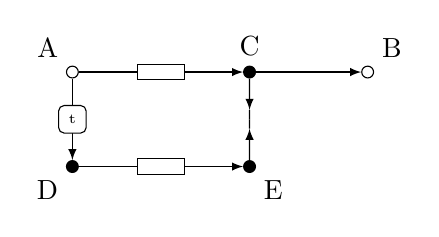
\begin{tikzpicture}[x=1.5cm, y=1.2cm]
        \node[node0, label=above left:A] (A) at (0, 0) {};
        \node[node0, label=above right:B] (B) at (2.5, 0) {};
        \node[node1, label=above:C] (C) at (1.5, 0) {};
        \node[node1, label=below left:D] (D) at (0, -1) {};
        \node[node1, label=below right:E] (E) at (1.5, -1) {};

        \chanFifoOne{A}{C}
        \chanTimert{A}{D}{t}
        \chanFifoOne{D}{E}
        \chanSyncDrain{C}{E}
        \chanSync{C}{B}
        
    \end{tikzpicture}
\end{minipage}
\hfill
\begin{minipage}{0.48\textwidth}
    \centering
    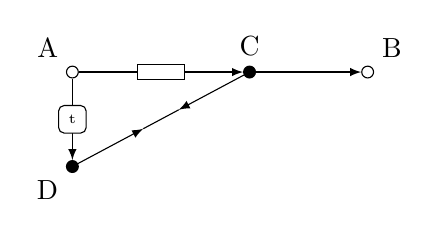
\begin{tikzpicture}[x=1.5cm, y=1.2cm]

        \node[node0, label=above left:A] (A) at (0, 0) {};
        \node[node0, label=above right:B] (B) at (2.5, 0) {};
        \node[node1, label=above:C] (C) at (1.5, 0) {};
        \node[node1, label=below left:D] (D) at (0, -1) {};

        \chanFifoOne{A}{C}
        \chanTimert{A}{D}{t}
        \chanSyncDrain{C}{D}
        \chanSync{C}{B}

    \end{tikzpicture}
\end{minipage}

\vspace{0.5cm}
\hrule
\vspace{0.5cm}

% ============================================================
% test_time_02
% ============================================================
\subsection*{test time 02}
\vspace{0.2cm}

\begin{minipage}{0.48\textwidth}
    \centering
    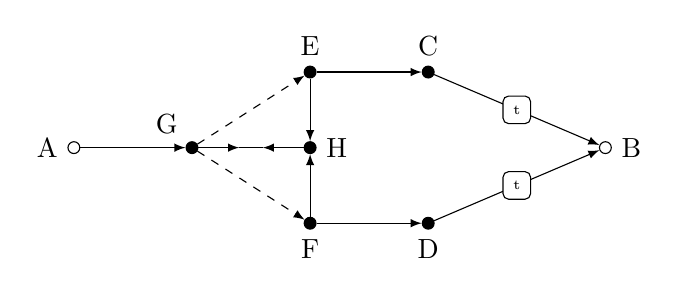
\begin{tikzpicture}[x=1.5cm, y=1.2cm]

        \node[node0, label=left:A] (A) at (0, 0) {};
        \node[node0, label=right:B] (B) at (4.5, 0) {};
        \node[node1, label=above left:G] (G) at (1, 0) {};
        \node[node1, label=above:E] (E) at (2, 0.8) {};
        \node[node1, label=above:C] (C) at (3, 0.8) {};
        \node[node1, label=below:F] (F) at (2, -0.8) {};
        \node[node1, label=below:D] (D) at (3, -0.8) {};
        \node[node1, label=right:H] (H) at (2, 0) {};

        \chanSync{A}{G}
        \chanLossySync{G}{E}
        \chanLossySync{G}{F}
        \chanSync{E}{H}
        \chanSync{F}{H}
        \chanSyncDrain{G}{H}
        \chanSync{E}{C}
        \chanSync{F}{D}
        \chanTimert{C}{B}{t}
        \chanTimert{D}{B}{t}
        
    \end{tikzpicture}
\end{minipage}
\hfill
\begin{minipage}{0.48\textwidth}
    \centering
    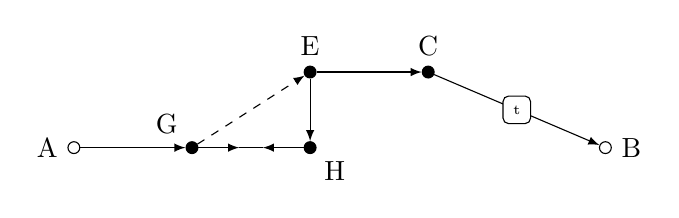
\begin{tikzpicture}[x=1.5cm, y=1.2cm]

        \node[node0, label=left:A] (A) at (0, 0) {};
        \node[node0, label=right:B] (B) at (4.5, 0) {};
        \node[node1, label=above left:G] (G) at (1, 0) {};
        \node[node1, label=above:E] (E) at (2, 0.8) {};
        \node[node1, label=below right:H] (H) at (2, 0) {};
        \node[node1, label=above:C] (C) at (3, 0.8) {};

        \chanSync{A}{G}
        \chanLossySync{G}{E}
        \chanSync{E}{H}
        \chanSyncDrain{G}{H}
        \chanSync{E}{C}
        \chanTimert{C}{B}{t}

    \end{tikzpicture}
\end{minipage}

\vspace{0.5cm}
\hrule
\vspace{0.5cm}

% ============================================================
% test_time_03
% ============================================================
\subsection*{test time 03}
\vspace{0.2cm}

\begin{minipage}{0.48\textwidth}
    \centering
    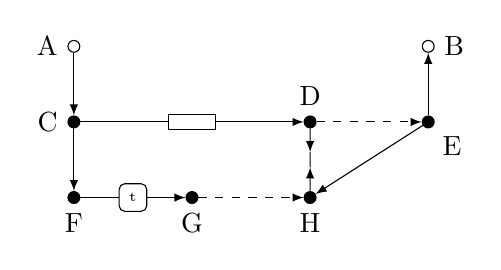
\begin{tikzpicture}[x=1.5cm, y=1.2cm]

        \node[node0, label=left:A] (A) at (0, 0.8) {};
        \node[node0, label=right:B] (B) at (3, 0.8) {};
        \node[node1, label=left:C] (C) at (0, 0) {};
        \node[node1, label=above:D] (D) at (2, 0) {};
        \node[node1, label=below right:E] (E) at (3, 0) {};
        \node[node1, label=below:F] (F) at (0, -0.8) {};
        \node[node1, label=below:G] (G) at (1, -0.8) {};
        \node[node1, label=below:H] (H) at (2, -0.8) {};

        \chanSync{A}{C}
        \chanFifoOne{C}{D}
        \chanSync{C}{F}
        \chanTimert{F}{G}{t}
        \chanLossySync{G}{H}
        \chanLossySync{D}{E}
        \chanSync{E}{H}
        \chanSyncDrain{D}{H}
        \chanSync{E}{B}
        
    \end{tikzpicture}
\end{minipage}
\hfill
\begin{minipage}{0.48\textwidth}
    \centering
    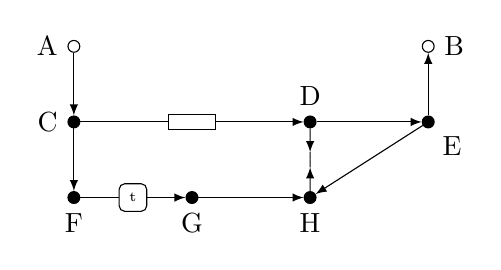
\begin{tikzpicture}[x=1.5cm, y=1.2cm]
        
        \node[node0, label=left:A] (A) at (0, 0.8) {};
        \node[node0, label=right:B] (B) at (3, 0.8) {};
        \node[node1, label=left:C] (C) at (0, 0) {};
        \node[node1, label=above:D] (D) at (2, 0) {};
        \node[node1, label=below right:E] (E) at (3, 0) {};
        \node[node1, label=below:F] (F) at (0, -0.8) {};
        \node[node1, label=below:G] (G) at (1, -0.8) {};
        \node[node1, label=below:H] (H) at (2, -0.8) {};

        \chanSync{A}{C}
        \chanFifoOne{C}{D}
        \chanSync{C}{F}
        \chanTimert{F}{G}{t}
        \chanSync{G}{H}
        \chanSync{D}{E}
        \chanSync{E}{H}
        \chanSyncDrain{D}{H}
        \chanSync{E}{B}

    \end{tikzpicture}
\end{minipage}

\vspace{0.5cm}
\hrule
\vspace{0.5cm}

\newpage
\section{Probablistic test cases}

\vspace{0.5cm}
\hrule
\vspace{0.5cm}

% ============================================================
% test_prob_01
% ============================================================
\subsection*{test prob 01}
\vspace{0.2cm}

\begin{minipage}{0.48\textwidth}
    \centering
    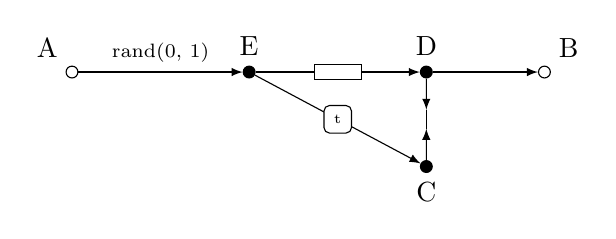
\begin{tikzpicture}[x=1.5cm, y=1.2cm]

        \node[node0, label=above left:A] (A) at (0, 0) {};
        \node[node0, label=above right:B] (B) at (4, 0) {};
        \node[node1, label=below:C] (C) at (3, -1) {};
        \node[node1, label=above:D] (D) at (3, 0) {};
        \node[node1, label=above:E] (E) at (1.5, 0) {};

        \chanRdmSync{A}{E}{rand(0, 1)}
        \chanFifoOne{E}{D}
        \chanTimert{E}{C}{t}
        \chanSyncDrain{C}{D}
        \chanSync{D}{B}

    \end{tikzpicture}
\end{minipage}
\hfill
\begin{minipage}{0.48\textwidth}
    \centering
    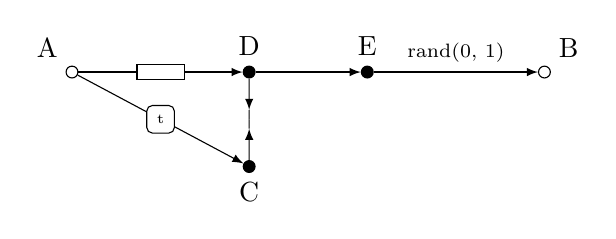
\begin{tikzpicture}[x=1.5cm, y=1.2cm]
        
        \node[node0, label=above left:A] (A) at (0, 0) {};
        \node[node0, label=above right:B] (B) at (4, 0) {};
        \node[node1, label=below:C] (C) at (1.5, -1) {};
        \node[node1, label=above:D] (D) at (1.5, 0) {};
        \node[node1, label=above:E] (E) at (2.5, 0) {};

        \chanSync{D}{E}
        \chanFifoOne{A}{D}
        \chanTimert{A}{C}{t}
        \chanSyncDrain{C}{D}
        \chanRdmSync{E}{B}{rand(0, 1)}

    \end{tikzpicture}
\end{minipage}

\vspace{0.5cm}
\hrule
\vspace{0.5cm}

% ============================================================
% test_prob_02
% ============================================================
\subsection*{test prob 02}
\vspace{0.2cm}

\begin{minipage}{0.48\textwidth}
    \centering
    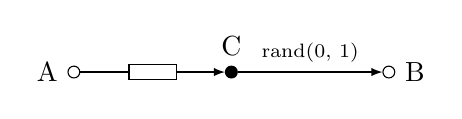
\begin{tikzpicture}[node distance=2cm]
        
        \node[node0, label=left:A] (A) at (0,0) {};
        \node[node1, label=above:C] (C) at (2,0) {};
        \node[node0, label=right:B] (B) at (4,0) {};

        \chanFifoOne{A}{C}
        \chanRdmSync{C}{B}{rand(0, 1)}

    \end{tikzpicture}
\end{minipage}
\hfill
\begin{minipage}{0.48\textwidth}
    \centering
    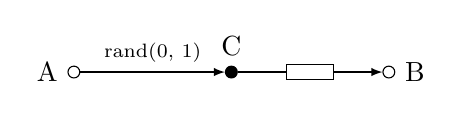
\begin{tikzpicture}[node distance=2cm]
        
        \node[node0, label=left:A] (A) at (0,0) {};
        \node[node1, label=above:C] (C) at (2,0) {};
        \node[node0, label=right:B] (B) at (4,0) {};
        
        \chanRdmSync{A}{C}{rand(0, 1)}
        \chanFifoOne{C}{B}
    \end{tikzpicture}
\end{minipage}

\vspace{0.5cm}
\hrule
\vspace{0.5cm}

% ============================================================
% test_prob_03
% ============================================================
\subsection*{test prob 03}
\vspace{0.2cm}

\begin{minipage}{0.48\textwidth}
    \centering
    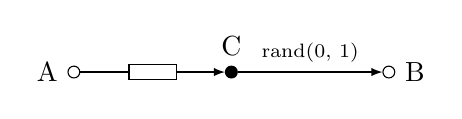
\begin{tikzpicture}[node distance=2cm]
        
        \node[node0, label=left:A] (A) at (0,0) {};
        \node[node1, label=above:C] (C) at (2,0) {};
        \node[node0, label=right:B] (B) at (4,0) {};
        
        \chanFifoOne{A}{C}
        \chanRdmSync{C}{B}{rand(0, 1)}

    \end{tikzpicture}
\end{minipage}
\hfill
\begin{minipage}{0.48\textwidth}
    \centering
    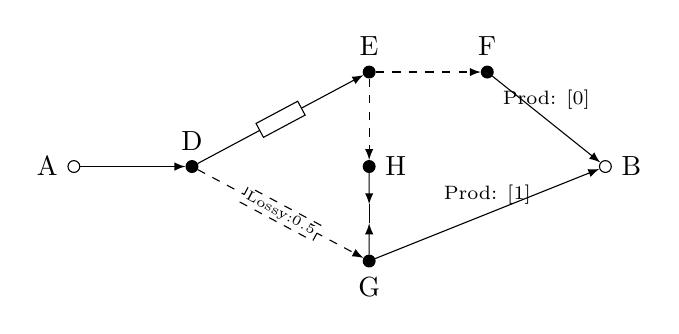
\begin{tikzpicture}[x=1.5cm, y=1.2cm]
        
        \node[node0, label=left:A] (A) at (0,0) {};
        \node[node0, label=right:B] (B) at (4.5,0) {};
        \node[node1, label=above:D] (D) at (1,0) {};
        \node[node1, label=above:E] (E) at (2.5, 1) {};
        \node[node1, label=above:F] (F) at (3.5, 1) {};
        \node[node1, label=right:H] (H) at (2.5, 0) {};
        \node[node1, label=below:G] (G) at (2.5, -1) {};
        
        \chanSync{A}{D}
        \chanFifoOne{D}{E}
        \chanLossySync{E}{F}
        \chanLossySync{E}{H}
        \chanProducerP{F}{B}{[0]}
        \chanLossyFifoOne{D}{G}{0.5}
        \chanProducerP{G}{B}{[1]}
        \chanSyncDrain{G}{H}
        
    \end{tikzpicture}
\end{minipage}

\vspace{0.5cm}
\hrule
\vspace{0.5cm}

% ============================================================
% test_prob_04
% ============================================================
\subsection*{test prob 04}
\vspace{0.2cm}

\begin{minipage}{0.48\textwidth}
    \centering
    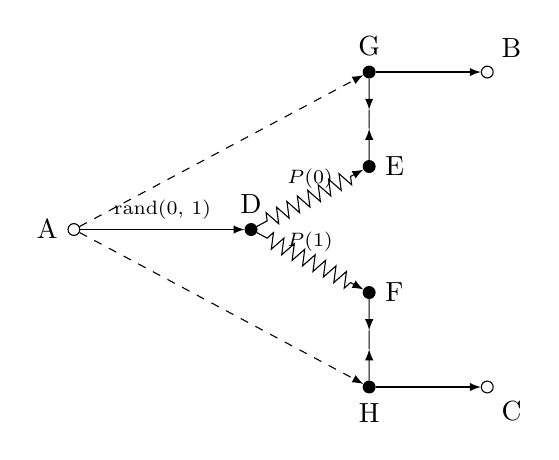
\begin{tikzpicture}[x=1.5cm, y=1cm]
        
        \node[node0, label=left:A] (A) at (-0.5,0) {};
        \node[node0, label=above right:B] (B) at (3, 2) {};
        \node[node0, label=below right:C] (C) at (3, -2) {};
        \node[node1, label=above:D] (D) at (1, 0) {};
        \node[node1, label=right:E] (E) at (2, 0.8) {};
        \node[node1, label=above:G] (G) at (2, 2) {};
        \node[node1, label=right:F] (F) at (2, -0.8) {};
        \node[node1, label=below:H] (H) at (2, -2) {};
        
        \chanRdmSync{A}{D}{rand(0, 1)}
        \chanLossySync{A}{G}
        \chanLossySync{A}{H}
        \chanFilterP{D}{E}{0}
        \chanFilterP{D}{F}{1}
        \chanSyncDrain{E}{G}
        \chanSyncDrain{F}{H}
        \chanSync{G}{B}
        \chanSync{H}{C}
        
    \end{tikzpicture}
\end{minipage}
\hfill
\begin{minipage}{0.48\textwidth}
    \centering
    \begin{tikzpicture}[x=1.5cm, y=1cm]
        
        \node[node0, label=left:A] (A) at (0,0) {};
        \node[node0, label=right:B] (B) at (3, 1) {};
        \node[node0, label=right:C] (C) at (3, -1) {};
        
        \chanProbLossy{A}{B}{0.5}
        \chanProbLossy{A}{C}{0.5}
        
    \end{tikzpicture}
\end{minipage}

\vspace{0.5cm}
\hrule
\vspace{0.5cm}

\end{document}